\chapter{Metoder til valg af model}
I dette kapitel vil vi redegøre for nogle metoder, som anvendes til at udvælge den ``bedste'' model. 
Vi er interesseret i en model, der er god til at prædiktere, men uden at være for kompleks.

Datasættet opdeles i en træningsmængde og en testmængde. 
Observationerne i træningsmængden betragtes som in-sample observationer og anvendes primært til at identificere modellen og estimere parametrene. 
Observationerne i testmængden betragtes som out-of-sample observationer og anvendes til at vurdere modellem, som er fundet udfra in-sample observationerne. 
 
\section{In-sample metoder}
For faktor modellen skal vi bestemme antallet af faktorer og for lasso modellen og dens generaliseringer skal vi estimere tuning parameteren.

\subsection{Valg af antal faktorer}
Antallet af faktorer kan bestemmes udfra informationskriterier, som betragter et tradeoff mellem at inkludere en ekstra faktor, dvs en ekstra parameter i modellen, mod omkostningen af at øge variabiliteten, som kommer af at estimere en ekstra parameter.
AIC kan anvendes til at udvælge antallet af faktorer, men \citep{Bai_Ng} beviset, at dette ikke giver et konsistent estimat.
Istedet foreslås at betragtet funktionen i \eqref{eq:dfm11}, som en funktion af \(\widehat{\tF}\) og \(k\), hvor \(0<k<k_\text{max}\) er antallet af faktorer, dvs
\begin{align*}
V \del{k, \widehat{\tF}} = \del{p T}^{-1} \sum_{j=1}^p \sum_{t=1}^{T} \del{x_{jt} -\boldsymbol{\lambda}_j \widehat{\tF}_t}^2
\end{align*}
som sammen med en straffunktion \(g \del{p,T}\) giver informationskriteriet
\begin{align*}
\text{IC} \del{k} = \ln V \del{k, \widehat{\tF}} + k g \del{p,T}.
\end{align*}
\citep{Bai_Ng} foreslår følgende straffunktioner
\begin{align}
g_1 \del{p,T} &= \frac{p + T}{p T} \ln \del{\frac{p T}{p + T}}, \label{eq:ic1} \\
g_2 \del{p,T} &= \frac{p + T}{p T} \ln \del{ \min \cbr{p, T}}, \label{eq:ic2} \\
g_3 \del{p,T} &= \frac{\ln \del{\min \cbr{p, T}}}{\min \cbr{p, T}},\label{eq:ic3}
\end{align}
som betegnes henholdsvis \(\text{IC}_1 \del{k}\), \(\text{IC}_2 \del{k}\) samt \(\text{IC}_3 \del{k}\). Disse giver konsistent estimation af antallet af faktorer i faktor modellen.

For \(p = T\) fås at \(g_2 \del{T,T} = 2 T^{-1} \ln \del{T}\), som bekendt er \(2\) gange straffaktoren for BIC.

\subsection{Udregning og valg af tuning parametre}
I dette underafsnit introduceres krydsvalidering og BIC, som anvendes til at estimere tuning parameteren \(\lambda\) i lasso modellen og den generaliseringer.
For elastisk net problemet \eqref{eq:4.2} betragtes to tuning parametre \(\lambda\) og \(\alpha\).

\subsubsection{Krydsvalidering}
\textit{En af de simpleste og oftest anvendte metoder til at estimere prædiktions fejlen er krydsvalidering. 
Dette afsnit giver en kort introduktion af krydsvalidering og er baseret på s. 175-184 i \citep{james}.}

%Krydsvalidering er en metode hvor vi estimerer prædiktions fejl fra træningssættet ved at holde fast i en del mængde. Delmængden bliver så anvendt som valideringssæt. 
%
%Denne tilgang med at anvende et valideringssæt er en simple strategi for at estimerer prædiktions fejl på en mængde af observationer. 

%Tilgangen splitter tilfældige observationer ind  i to delmængder, et træningssæt og et valideringssæt. 
%Forskellige regressions modeller fittes på træningsdata og deres prædiktion af responsvariablen er evaluerede i valideringssættet. 
%Valideringssættets fejl er normalt målt i MSE. 
%Tilgangen med anvendelse af et valideringssæt er nem at implementere, men den har to ulemper. 
%\begin{itemize}
%\item Prædiktions fejlene kan være meget varierende, da fejlene afhænger af hvilken observationer der er inkluderet i træningssættet og valideringsættet. 
%\item Idet denne tilgang deler vores data op i to delmængder vil vi derfor have færre observationer til at fitte vores model på. Derudover performere statistiske metoder sig dårligere på et træningsdata med færre informationer. Derfor kan valideringsættets have en tendens til at overestimere prædiktions fejlene for modellen, som er fitted på hele datasættet. ??
%\end{itemize}
%For at undgå disse to problemstillinger introduceres k-fold krydsvalidering. 

%\subsubsection{k-fold krydsvalidering}
En k-fold krydsvalidering opdeler tilfældigt observationerne i \(k\) grupper, som er tilnærmelsesvis af samme størrelse.
Én af disse grupper anvendes som valideringsmængde, og de resterende \(k-1\) grupper betragtes som træningsmængde.
En regressions model fittes på træningsmængden, hvorfra den gennemsnitlige kvadrerede fejl findes udfra valideringsmængden, hvilket giver \(\text{MSE}_1\).
Denne procedure gentages \(k\) gange, således at hver gruppe betragtes som valideringsmængde.
Dette resulterer i \(k\) estimater af prædiktions fejlen $\text{MSE}_1, \text{MSE}_2, \dots , \text{MSE}_k$.
Estimatet for \(k\)-fold krydsvalidering er da givet ved
\begin{align}
\text{CV}_k = \frac{1}{k} \sum_{i=1}^k \text{MSE}_i. \label{eq:cv_k}
\end{align}
Oftest er $k=5$ eller $k = 10$. 
Figur \ref{fig:cv_teori} illustrerer en 5-fold krydsvalidering. 
%
\begin{figure}
\center
\scalebox{0.6}{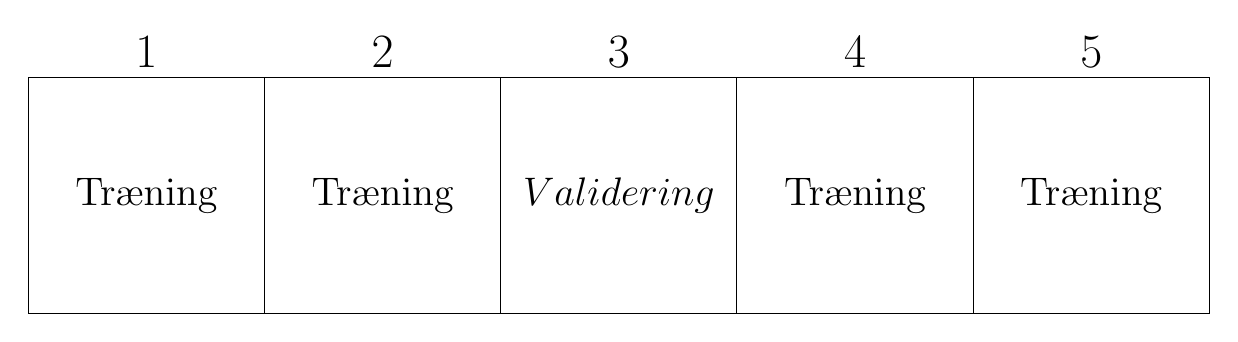
\begin{tikzpicture}
%\filldraw [green] (-3,0) circle (2pt) node [below, black]{$\widehat{\tmu}_0$};
\draw [-] (0,0) -- (15,0);
\draw [-] (0,3) -- (15,3);

\draw [-] (0,0) -- (0,3);
\draw [-] (15,0) -- (15,3);
\draw [-] (3,0) -- (3,3);
\draw [-] (6,0) -- (6,3);
\draw [-] (9,0) -- (9,3);
\draw [-] (12,0) -- (12,3);


\node[above] at (1.5,3) {\LARGE 1};
\node[above] at (4.5,3) {\LARGE2};
\node[above] at (7.5,3) {\LARGE3};
\node[above] at (10.5,3) {\LARGE4};
\node[above] at (13.5,3) {\LARGE5};

\node[align=left] at (1.5,1.5) {\Large Træning};
\node[align=left] at (4.5,1.5) {\Large Træning};
\node[align=left] at (7.5,1.5) {\Large $\text{Validering}$};
\node[align=left] at (10.5,1.5) {\Large Træning};
\node[align=left] at (13.5,1.5) {\Large Træning};

%\draw [<-] (1,4) node [above] {$\x_2$} --(-3,0);
%\draw [<-] (-5,4) node [above] {$\x_3$} --(-3,0);

\end{tikzpicture}}
\caption{5-fold krydsvalidering. I dette tilfælde fittes modellen i første, anden, fjerde og femte gruppe af data og udregner prædiktionsfejlen af den fittede model for tredje gruppe.} \label{fig:cv_teori}
\end{figure} 
%
Et $k$-fold krydsvalidering har en lav varians, da \eqref{eq:cv_k} tager det gennemsnitlige output af $k$ fittede modeller, som har en lav korrelation, siden vi har et relativt lille overlap mellem træningsmængden i hver model. 
Bias kunne være et problem i forhold til hvordan vi vælger vores træningsmængde. Hvis vi ikke har nok observationer i træningsmængden vil $k$-fold krydsvalidering have høj bias. Derfor er der også en bias-varians trade-off med valget af $k$. 

\subsubsection{BIC}
Tuning parametrene kan også vælges udfra Bayesian informationskriteriet.
Vi betragter dens skalerede version
%
%\begin{defn}[Bayesian informationskriteriet (BIC)] \label{def:bic}
\begin{align*}
\text{BIC} =  \frac{- 2 \widehat{\ell}}{T} + \frac{p \log T}{T}, 
\end{align*}
hvor \(\widehat{\ell}\) er den maksimerede log-likehood, \(p\) er antallet af parametre og \(T\) er antallet af observationer i træningsmængden.
%\end{defn} 
%
%BIC vil være større des lavere log-likehood eller jo flere parametre der er i modellen.
Modellen med den laveste BIC vælges, da det indikerer, at modellen giver en god tilnærmelse af data i forhold til modellens kompleksitet. 

Lad fejlledene være iid og normalfordelte, da er maksimum likelihood estimatoren for variansen defineret som
\begin{align*}
\widehat{\sigma}_p^2 = \frac{1}{T} \sum_{t=1}^{T} \del{y_t - \sum_{j=1}^p x_{tj}\beta_j}^2,
\end{align*}
og BIC kan omskrives til
\begin{align*}
\text{BIC} = \log \widehat{\sigma}^2_p + \frac{p \log T}{T}.
\end{align*}

\section{Out-of-sample metoder}
Vi anvender et rolling scheme forecast med expanding estimerings windows. 
Dvs at det første estimerings window indeholder altså de sande observationer fra tiden 1 til tid $t$, og den næste estimerings window indeholderde sande observationer fra tiden 1 til $t+1$.
Den første rolling window indeholder altså observationer fra tiden 1 til $m$, og den næste rolling window indeholder observationer fra periode 2 til $m+1$ og sådan fortsætter det. 

For at vurdere en models prædiktions evnen betragtes den gennemsnitlige kvadrede fejl (MSE) og den gennemsnitlige absolutte fejl (MAE), som er defineret ved
\begin{align}
\text{MSE} & =  \frac{1}{T} \sum_{t=1}^{T} \del{y_{t} - \widehat{y}_{t}}^2, \label{eq:mse}  \\
\text{MAE} & =  \frac{1}{T} \sum_{t=1}^{T} \abs{y_{t} - \widehat{y}_{t}}, \label{eq:mae} 
\end{align} 
hvor $T$ er antallet af observationer i testmængden, $y_{t}$ er observationen til tid $t$ og $\widehat{y}_{t}$ er prædiktionen af $y_{t}$.
MSE og MAE kan betragtes som tabsfunktioner, da de måler en afvigelse fra de observerede værdier.
Tabsfunktionerne vil være lig 0 for en perfekt prædiktion, og ellers vil de have en positiv værdi, derfor foretrækkes modeller med lav MSE eller MAE.

Foruden MSE og MAE betragtes \textit{Diebold-Mariano} testen samt \textit{model confidence set} (MCS) proceduren.
Diebold-Mariano testen kan anvendes til at teste om én model er signifikant bedre end en anden model, mens MCS proceduren identificerer en mængde af modeller, som er signifikant bedre end de øvrige modeller, men ikke signifikant bedre end de øvrige modeller i mængden.
Nedenfor introduceres kort Diebold-Mariano testen samt general teori for MCS.

\subsection{Diebold-Mariano testen}
Prædiktionen af to potentielle modeller kan testes imod hinanden med Diebold-Mariano testen.
Lad \(\widehat{y}_{i,t}\) og \(\widehat{y}_{j,t}\) være \(i\)'te og \(j\)'te models prædiktion af \(y_{t}\).
Tabet for model \(i\) til tid \(t\) betragtes ved tabsfunktionerne
\begin{align}
L \del{y_t, \widehat{y}_{i,t}} &= \abs{y_t - \widehat{y}_{i,t}} \label{eq:lossMAE} \\
L \del{y_t, \widehat{y}_{i,t}} &= \del{y_t - \widehat{y}_{i,t}}^2. \label{eq:lossMSE}
\end{align}
Differencen mellem tabsfunktionerne af model \(i\) og \(j\) er givet ved 
\begin{align*}
d_{ij,t} = L \del{y_t, \widehat{y}_{i,t}} - L \del{y_t, \widehat{y}_{j,t}}.
\end{align*}
%
\begin{defn}[Diebold-Mariano test]
Betragt \(\hyp_0 : \E{d_{ij,t}} = 0\) imod \(\hyp_A: \E{d_{ij,t}} \neq 0\). Teststørrelsen for DM testen er defineret som følgende
\begin{align*}
\text{DM} = \frac{\bar{d}_{ij}}{\sqrt{\widehat{\mathrm{Var}}\!\sbr{\bar{d}_{i.}}}} =  \frac{\bar{d}_{ij}}{\sqrt{\frac{\widehat{\text{LRV}}_{\bar{d}_{ij}}}{n}}},
\end{align*}
hvor $\bar{d} = \frac{1}{T_0} \sum^{T}_{t = t_0} d_{t +1} $ og $\text{LRV}_{\bar{d}} = \gamma_0 + 2\sum_{j = 1}^{\infty} \gamma_j$, hvor $\gamma_j = \Cov{d_{t +1}}{d_{t+1-j}}$. 
\end{defn}
%
Det kan vises, at DM teststørrelsen er asymptotisk standard normalfordelt under nulhypotesen. Derfor afvises nulhypotesen ved niveau $5 \%$, hvis $\abs{\text{DM}} > 1.96$
\subsection{Model Confidence Set}
Dette afsnit er baseret på \citep{mcs2011}. 
MCS proceduren identificerer en mængde af modeller, hvori den ``bedste'' model er indeholdt givet et niveau af confidence.
I modsætning til andre modeludvælgelses kriterier, vælger MCS proceduren en mængde af modeller.
Hvis mængden blot indeholder én model, da er modellen signifikant bedre end de øvrige modeller.
Proceduren kræver ikke en benchmark model, da alle modellerne testes imod hinanden.

Vi betragter en endelig mængde af indekser \(\mathcal{M}_0 = \cbr{1, \ldots, m_0}\), hvor hvert indeks svarer til en model.
Lad \(y_t\) være den observerede værdi til tid \(t\) og lad \(\widehat{y}_{i,t}\) være \(i\)'te models prædiktion af \(y_t\).  

Tabet for model \(i\) til tid \(t\) betragtes ved en given tabsfunktion \(L \del{y_t, \widehat{y}_{i,t}}\), hvor den absolutte og kvadrede fejl igen betragtes, som er givet i \eqref{eq:lossMAE} og \eqref{eq:lossMSE}.
Differencen mellem tabsfunktionerne af model \(i\) og \(j\) er givet ved
\begin{align*}
d_{ij,t} = L \del{y_t, \widehat{y}_{i,t}} - L \del{y_t, \widehat{y}_{j,t}}, \quad i, j \in \mathcal{M}_0, \quad t = 1, \ldots, T.
\end{align*}
Vi antager, at \(\mu_{ij} = \E{d_{ij,t}}\) er endelig og uafhængig af \(t\) for alle \( i, j \in \mathcal{M}_0\).
Modellerne rangeres efter forventet tab, således at model \(i\) foretrækkes frem for model \(j\) hvis \(\mu_{ij} < 0\).
%
\begin{defn}[Mængden af superior modeller]
Mængden af superior modeller defineres som
\begin{align*}
\mathcal{M}^* \equiv \cbr{i \in \mathcal{M}_0 : \mu_{ij} \leq 0, \quad \forall j \in \mathcal{M}_0}. 
\end{align*}
\end{defn}
%
MCS estimeres ved sekventielt at trimme mængden af potentielle modeller, \(\mathcal{M}_0\).
I hvert step tester proceduren følgende nulhypotese
\begin{align*}
\hyp_0: \mu_{ij} = 0, \quad \forall i,j \in \mathcal{M},
\end{align*}
for en mængde af modeller \(\mathcal{M} \subset \mathcal{M}_0\).
Nulhypotesen testes imod den alternative hypotese \(\hyp_A: \mu_{ij} \neq 0\) for nogle \(i, j \in \mathcal{M}\).
Den første test er for den fulde mængde af modeller, dvs \(\mathcal{M} = \mathcal{M}_0\), hvis \(\hyp_0\) afvises, da elimineres den dårligste model fra \(\mathcal{M}\).
Testen gentages indtil første gang nulhypotesen ikke kan afvises, og den resterende mængde af modeller er da den estimerede MCS, \(\widehat{\mathcal{M}}^*\).
Med et fast \(\alpha\), da konstrueres et \(\del{1-\alpha}\)-konfidensmængde, \(\widehat{M}^*_{1-\alpha}\), for de bedste modeller i \(\mathcal{M}_0\).

\subsubsection{Tests konstrueret fra bootstrap}
I dette afsnit introduceres to tests, som er baseret på multiple \(t\)-teststørrelser, som findes ud fra bootstrap.
Definer \(\bar{d}_{ij} = \frac{1}{T} \sum_{t = 1}^T d_{ij,t}\) og \(\bar{d_{i.}} = \frac{1}{m} \sum_{j \in \mathcal{M}} \bar{d}_{ij}\) for \(i,j \in \mathcal{M}\), hvor \(\bar{d}_{ij}\) måler det relative empiriske tab mellem model \(i\) og \(j\) og \(\bar{d_{i.}}\) er det empiriske tab af model \(i\) relativ til gennemsnittet af modellerne i \(\mathcal{M}\). 
Herudfra konstrueres \(t\)-teststørrelserne
\begin{align}
t_{ij} = \frac{\bar{d}_{ij}}{\sqrt{\widehat{\mathrm{Var}}\!\sbr{\bar{d}_{ij}}}} \quad \text{og} \quad t_{i.} = \frac{\bar{d}_{i.}}{\sqrt{\widehat{\mathrm{Var}}\!\sbr{\bar{d}_{i.}}}}, \quad \text{for } i,j \in \mathcal{M}, \label{eq:t_statistics}
\end{align}
hvor \(\widehat{\mathrm{Var}}\!\sbr{\bar{d}_{ij}}\) and \(\widehat{\mathrm{Var}}\!\sbr{\bar{d}_{i.}}\) er estimater af henholdsvis \(\Var{\bar{d}_{ij}}\) og \(\Var{\bar{d}_{i.}}\), som findes udfra bootstrap.
%----
%For at udregne disse bootstraped varianser\(\widehat{\mathrm{Var}}\!\sbr{\bar{d}_{i.}}\), udfører vi en block-bootstrap procedure af \(B\) resamples (for some large integer \(B\)), where the block length \(p\) is the max number of significants parameters obtained by fitting an AR\((p)\) process on all the \(d_{ij}\) terms. ----

Teststørrelserne er da givet ved
\begin{align} 
T_R = \max_{i,j \in \mathcal{M}} \abs{t_{ij}} \quad \text{og} \quad T_{\text{max}} = \max_{i \in \mathcal{M}} t_i. \label{eq:test_statistics}
\end{align}
hvor \(t_{ij}\) og \(t_i.\) er givet i \eqref{eq:t_statistics}.
Teststørrelserne i \eqref{eq:test_statistics} anvendes til at teste følgende nulhypoteser
\begin{align*}
\mathcal{H}_{ij}:\mu_{ij}&=0, \\
\mathcal{H}_{i.} : \mu_{i.}&=0,
\end{align*}
hvor \(\mu_{ij} = \E{\bar{d}_{ij}}\) og \(\mu_{i.} = \E{\bar{d}_{i.}}\).
De asymptotiske fordelinger af disse teststørrelser er ikke-standard, da de afhænger af støjparametre under både nulhypotesen og den alternative hypotese.

